\documentclass{report}
\usepackage{amsmath,amsthm,amssymb}
\usepackage{mathtext}
\usepackage[T1,T2A]{fontenc}
\usepackage[utf8]{inputenc}
\usepackage[russian, english]{babel}
\usepackage{graphicx}

\begin{document}


\section*{Лабораторная работа №7. Задача Коши}
Выполнил студент группы 428 Берсенев Даниил Романович
\section*{Вариант №17}
Решить методом Тейлора 2-го порядка задачу Коши
$$y''+ 16y'-16y= sin(4x)exp(x)$$ с заданной относительной точностью 0.01. Требуется построение графиков решения $y(x), y'(x)$, а также фазовых траекторий.
\section*{Теоретическая часть}
Простейшим способом построения приближенного решения задачи Коши в точке $x_{n+1}$ сетки является способ, основанный на разложении решения в ряд Тейлора в предыдущей точке сетки $x_n$ по степеням шага $h$: $$y(x_{n+1}) = y(x_n) + h \varphi_p (x_n, y_n, h),$$ $$\varphi_p (x_n, y_n, h) = y'(x) + \cfrac{h}{2} y''(x) + \dots + \cfrac{h^{p-1}}{p!} y^{(p)}(x)$$При p = 2 получаем метод Тейлора 2-го порядка. Для каждой i-ой итерации будем искать $$\begin{cases} y_{i+1} = y_i + h y'_i + \cfrac{h^2}{2!}y''_i + \cfrac{h^3}{3!}y'''_i \\
y'_{i+1} = y'_i + hy''_i + \cfrac{h^2}{2!}y'''_i \\
y''_{i+1} = sin(4x)\exp(x) - 16y'_i +16y \\
y'''_{i+1} = 4cos(4x)\exp(x)+\exp(x)sin(4x) - 16y''_i + 16y'_i \\
\end{cases}$$
\section*{Практическая часть}
Функция void taylor(double h, double *y, double *dy) заносит решение, найденное методом Тейлора в массивы y и dy, double find\_shag(double eps) нужна для отыскания шага, оптимального для обеспечения определенной погрешности. Вывод данных осуществляется в файл data.dat.
\section*{Результаты}
В результате работы программы было найденно решение задачи Коши. Оно представленно на рисунках ниже, где также проиллюстрированы фазовые траектории.

\begin{figure}[h]
    \centering
    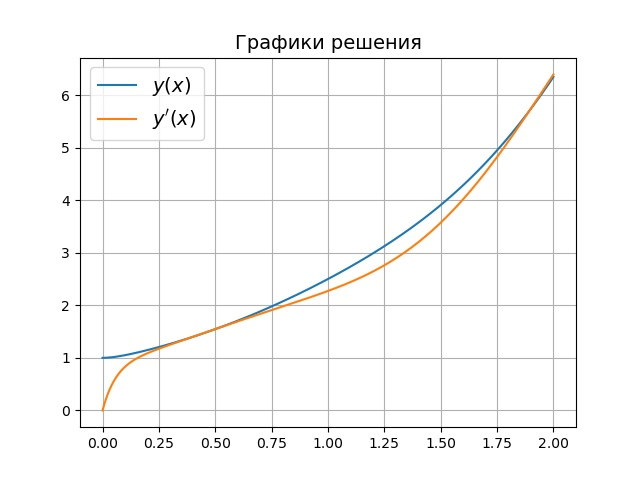
\includegraphics[width=14cm]{reshenie.jpg}
\end{figure}

\begin{figure}[h]
    \centering
    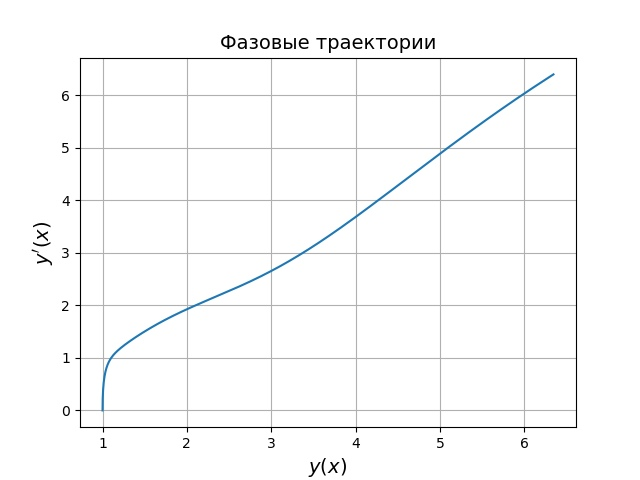
\includegraphics[width=14cm]{faz.jpg}
\end{figure}
\end{document}
